\documentclass[Japanese,noauthor]{dicomopapers}

\usepackage[dvipdfmx]{graphicx}
\usepackage{latexsym}
\usepackage{amsmath}
\usepackage{booktabs}
\usepackage{multirow}
\usepackage{amssymb}
\usepackage{textcomp}
\usepackage{tikz}
\usetikzlibrary{arrows,positioning,fit,backgrounds,calc}

\def\Underline{\setbox0\hbox\bgroup\let\\\endUnderline}
\def\endUnderline{\vphantom{y}\egroup\smash{\underline{\box0}}\\}
\def\|{\verb|}

\begin{document}

% 和文表題
\title{AFAD: 計算・モデル二重異種性に対応する\\適応的連合アーキテクチャ分散学習}

% 英文表題
\etitle{AFAD: Adaptive Federated Architecture Distribution\\for Dual Heterogeneity in Federated Learning}

% 所属ラベルの定義
\affiliate{OIT}{大阪工業大学 大学院 情報科学研究科\\Graduate School of Information Science, Osaka Institute of Technology}


\author{島野 凌}{RYO SHIMANO}{OIT}
\author{須山 敬之}{TAKAYUKI SUYAMA}{OIT}

\begin{abstract}
  連合学習（Federated Learning; FL）の実環境では，端末ごとに計算能力が異なる「計算異種性」と，
  CNN や Transformer など異なるモデル構造を持つ「アーキテクチャ異種性」が同時に存在する．
  既存手法の HeteroFL は計算異種性のみ，FedGen はアーキテクチャ異種性のみに対応しており，
  著者らの知る限り，両者を同時に解決する手法は存在しなかった．
  本稿では，32次元共有ボトルネック層を接点として HeteroFL と FedGen を統合した
  フレームワーク AFAD（Adaptive Federated Architecture Distribution）を提案する．
  すべての端末モデルが同一次元の潜在表現を共有することで，
  異なる幅・異なるアーキテクチャを持つ端末が同一の FL 環境に参加できる．
  OrganAMNIST を用いた IID 環境での評価により，AFAD はサーバ精度 82.93\% を達成した．
  ViT 端末を含む全 10 台という，より困難な条件下でありながら，
  CNN 端末 5 台を対象とした HeteroFL（82.20\%）を上回り，
  二重異種性への同時対応が HeteroFL 比での精度低下を伴わないことを示した．
  FedGen（86.32\%）との差 3.4 ポイントは今後の課題として残るが，
  HeteroFL が参加を許容しない ViT 端末を含む全 10 台という
  より困難な設定でこの結果を達成した点は，提案手法の実用的価値を示す．
\end{abstract}

\maketitle

\section{はじめに}
%----------------------------------------------------------------------

近年，スマートフォンや医療機器，IoT センサなど多様な端末から生成されるデータを活用した
機械学習の需要が急速に高まっている．
しかしこれらのデータは高度に個人的であり，
プライバシーの観点から端末外へのデータ転送が困難または不可能なケースが多い．

こうした背景から，McMahan ら\cite{McMahanFedAvg}が提案した
連合学習（Federated Learning; FL）が注目を集めている．
FL はデータを端末内に保持したまま，各端末がローカルで学習したモデルパラメータのみをサーバと
共有することで，プライバシーを保護しつつ分散的な協調学習を実現する枠組みである．
医療診断，スマートフォンの次単語予測，スパム検出など幅広い応用が報告されている．

しかし実用的な FL 環境においては，2 種類の異種性が同時に存在するという問題がある．

\textbf{計算異種性（Computational Heterogeneity）}:
スマートフォン，タブレット，組み込みデバイスなど，
処理能力・メモリ容量が大きく異なる端末が混在する．
計算資源が限られた端末はフルサイズのモデルを実行できないため，
すべての端末が同一のモデルを用いる従来の FL 手法（FedAvg\cite{McMahanFedAvg}）では，
非力な端末が学習に参加できないという問題が生じる．

\textbf{アーキテクチャ異種性（Architectural Heterogeneity）}:
端末や組織ごとに異なるモデルアーキテクチャを採用するケースが増えている．
たとえば画像認識において，CNN ベースのモデルと
Vision Transformer（ViT）\cite{VisionTransformer}ベースのモデルが混在することは珍しくない．
異なるアーキテクチャ間では重みの構造が異なるため，
FedAvg のようなパラメータ平均による集約が直接適用できない．

既存の代表的手法はいずれか一方の異種性にしか対応できない（表~\ref{tab:related}）．
HeteroFL\cite{HeteroFL}は計算異種性を解決するが，
異なるアーキテクチャ間での知識共有を提供しない．
FedGen\cite{FedGen}はアーキテクチャ非依存の知識蒸留を実現するが，
全端末が同一サイズのモデルを持つことを前提としている．

本研究では，この空白を埋めるフレームワーク
AFAD（Adaptive Federated Architecture Distribution）を提案する．
AFAD は，32次元の共有ボトルネック層を介して HeteroFL と FedGen を統合することで，
計算異種性とアーキテクチャ異種性の両方を同時に扱う．
本稿の貢献を以下に示す．

\begin{itemize}
  \item 著者らの知る限り，計算異種性（モデル幅）とアーキテクチャ異種性（CNN/ViT）を
        同時に扱う最初の FL フレームワーク AFAD を提案する．
  \item 32次元共有ボトルネック層という単純な設計により，
        HeteroFL の重み集約機構と FedGen の知識蒸留機構を干渉を最小化して統合する設計を示す．
  \item OrganAMNIST を用いた IID 環境での実験により，
        AFAD がサーバ精度 82.93\% を達成し，HeteroFL（82.20\%）を上回ることを示す．
        二重異種性への同時対応が HeteroFL 比での精度低下を伴わないことを実証する．
\end{itemize}

%----------------------------------------------------------------------

\section{関連研究}
%----------------------------------------------------------------------

\subsection{連合学習の基礎}

FL の基礎アルゴリズムである FedAvg\cite{McMahanFedAvg}は，
各端末がローカルデータで複数エポック学習した後，
サーバがパラメータを加重平均によって集約するという手順を繰り返す．
シンプルで効果的な手法だが，全端末が同一アーキテクチャ・同一サイズのモデルを使用することを前提とする．

データの分布が端末間で偏る Non-IID 設定では，
FedAvg の収束が著しく低下することが理論的・実証的に示されている\cite{ZhaoNonIID,noniid_convergence}．

\subsection{計算異種性への対応}

計算能力の異なる端末が共存する環境への対応として，
Li ら\cite{FedProx}は端末のローカル更新を正則化する FedProx を提案した．
FedProx はフルモデルを用いたまま局所最適解への収束を抑制するが，
非力な端末が大きなモデルを実行しなければならないという制約は解決しない．

HeteroFL\cite{HeteroFL}はこの制約に正面から取り組む手法であり，
グローバルモデルの幅をチャネル・ニューロン単位で縮小し，
各端末の計算能力に応じたサブモデルを配布する．
例えば縮小率 $r = 0.5$ の端末は，グローバルモデルの各層のチャネル数を半分にしたモデルを受け取る．
集約時には，各パラメータを「そのパラメータを学習した端末の数（カウント）」で割って正規化する，
\textbf{カウントベース集約}を採用することで，
幅の異なるモデル間でも安定した重み平均が実現できる．
これにより，小さなモデルしか動かせない端末でも，
自身のモデルサイズの範囲内でグローバルモデルの学習に貢献できる（図~\ref{fig:heterofl_concept}）．

\begin{figure}[htb]
  \centering
  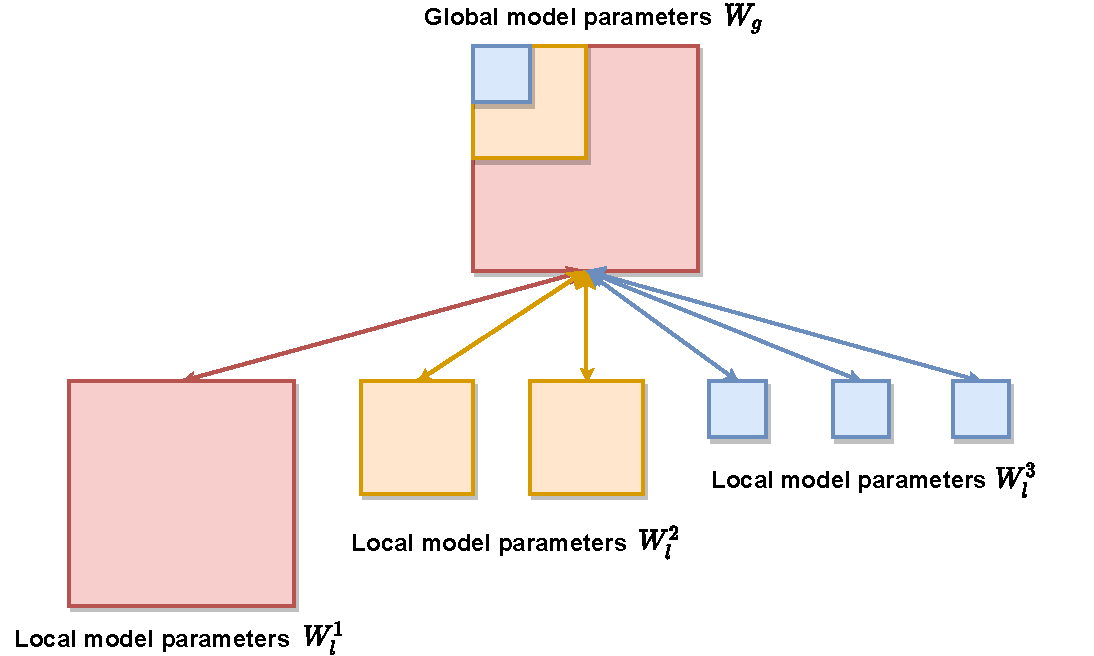
\includegraphics[width=\linewidth]{figs/heterofl_concept.pdf}
  \caption{HeteroFL における幅スケーリングとパラメータ配布
    （文献\cite{HeteroFL} の Figure 1 より引用）．
    グローバルモデル $W_g$（上段）のパラメータを，
    計算複雑度に応じた 3 段階（赤: 大，橙: 中，青: 小）のサブモデルとして
    6 台の端末に配布する．
    小さいモデルのパラメータはすべての端末が保持し，
    大きいモデルのみが持つパラメータは対応する端末のみが保持する．}
  \label{fig:heterofl_concept}
\end{figure}

一方，HeteroFL はすべての端末が同じアーキテクチャ（例: ResNet）を使うことを前提としており，
CNN の畳み込みカーネルと ViT のアテンション重みは構造が根本的に異なるため，
両者を混在させた学習には対応していない．

\subsection{アーキテクチャ異種性への対応}

異なるアーキテクチャ間での知識共有を実現するアプローチとして，
知識蒸留（Knowledge Distillation; KD）を活用した手法が複数提案されている．

Lin ら\cite{FedDF}は，各端末のモデルをアンサンブルし，
その出力を蒸留することで共有データセット上でサーバモデルを訓練する FedDF を提案した．
ただし FedDF はサーバ側での蒸留に公開データセットを必要とするという制約がある．

FedGen\cite{FedGen}はこの制約を克服し，
サーバ側に Generator を配置することで，外部データなしに知識蒸留を実現する．
FedGen の Generator が生成するのは生の画像ではなく，
\textbf{クラスラベルを条件とした仮想潜在ベクトル}——モデルの中間層特徴に相当する低次元ベクトル——である．
各端末はこの仮想潜在ベクトルを自身の分類器（最終層）に直接入力し，
その出力確率分布がサーバ側の複数端末モデルの予測の平均（アンサンブル出力）に近づくよう学習する．
仮想潜在ベクトルが「分類器への入力」として機能するため，
バックボーンのアーキテクチャが端末によって異なっていても同一の教師信号を使えるという点が，
アーキテクチャ非依存な知識共有を可能にする仕組みである（図~\ref{fig:fedgen_overview}）．

\begin{figure}[htb]
  \centering
  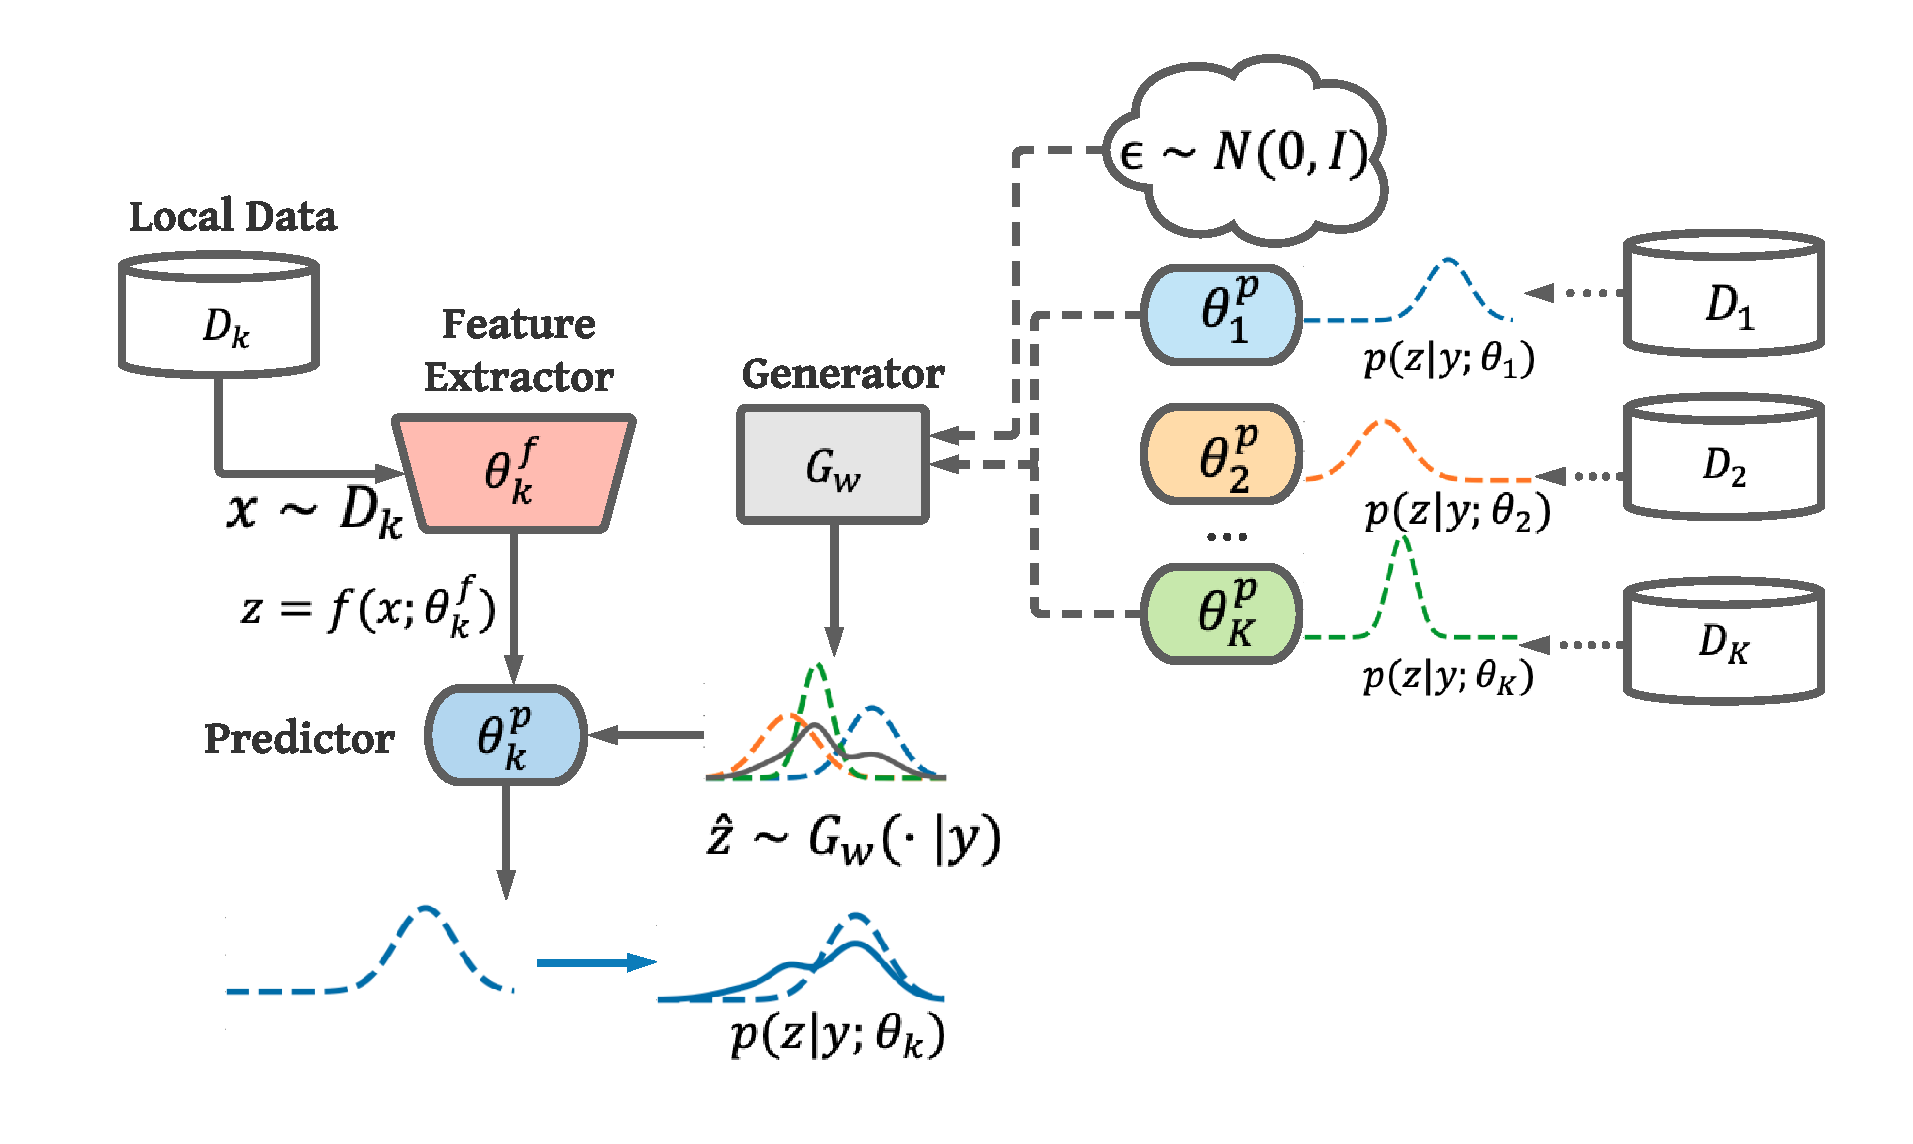
\includegraphics[width=\linewidth]{figs/fedgen_overview.pdf}
  \caption{FedGen のシステム概要
    （文献\cite{FedGen} の Figure 1 より引用）．
    サーバ上の Generator $G_\mathbf{w}$ が，
    各端末の Predictor（$\theta_k^p$）の予測分布に整合する
    仮想潜在ベクトル $\hat{z} \sim G_\mathbf{w}(\cdot|y)$ を生成する（右上）．
    各端末はこの仮想潜在ベクトルを自身の Predictor に入力し（左下），
    アンサンブル出力に近づくよう学習することで，
    外部データなしに端末間の知識蒸留を実現する．}
  \label{fig:fedgen_overview}
\end{figure}

しかし FedGen は全端末が同一サイズのモデルを持つことを前提としており，
端末間でモデルの幅（チャネル数）が異なる計算異種性への対応は考慮されていない．

\subsection{モデル集約の高度化}

Wang ら\cite{FedMA}はニューロンのパーミュテーション不変性を利用して
モデルをマッチングしながら集約する FedMA を提案した．
FedMA は同一アーキテクチャのモデル間での集約精度を向上させるが，
異なるアーキテクチャ間での適用は困難である．

\subsection{既存手法の整理}

表~\ref{tab:related}に，AFAD と関連手法の比較を示す．
計算異種性とアーキテクチャ異種性の両方を同時に扱う手法は，
AFAD 以前には存在しなかった．

\begin{table}[hbt]
  \centering
  \caption{連合学習関連手法の比較}
  \label{tab:related}
  \begin{tabular}{lp{1.2cm}p{1.5cm}p{1.2cm}}
    \toprule
    手法 & 計算\newline 異種性 & アーキテクチャ\newline 異種性 & 外部データ\newline 不要 \\
    \midrule
    FedAvg\cite{McMahanFedAvg}  & \texttimes & \texttimes & \checkmark \\
    FedProx\cite{FedProx}       & \texttimes & \texttimes & \checkmark \\
    HeteroFL\cite{HeteroFL}     & \checkmark & \texttimes & \checkmark \\
    FedDF\cite{FedDF}           & \texttimes & \checkmark & \texttimes \\
    FedGen\cite{FedGen}         & \texttimes & \checkmark & \checkmark \\
    \textbf{AFAD（提案手法）}       & \checkmark & \checkmark & \checkmark \\
    \bottomrule
  \end{tabular}
\end{table}

%----------------------------------------------------------------------

\section{提案手法: AFAD}
%----------------------------------------------------------------------

\subsection{設計方針}

\textbf{二重異種性を同時に解決する難しさ．}
HeteroFL と FedGen をそのまま組み合わせようとすると根本的な矛盾が生じる．
HeteroFL は計算異種性に対応するためにバックボーンの幅を端末ごとに縮小する．
その結果，バックボーンの出力次元が端末によって異なる（CNN $r=1.0$ なら512次元，$r=0.25$ なら128次元）．
FedGen の Generator はすべての端末の分類器に同じ仮想潜在ベクトルを渡す設計になっているため，
出力次元が統一されていない状態では正しく機能しない．
逆に FedGen のために全端末の出力次元を揃えようとすると，
幅スケーリングができなくなり計算異種性への対応が失われる．

\textbf{AFAD の解法：固定次元ボトルネックによる次元の統一．}
AFAD はこの矛盾を解決するため，バックボーンの直後に\textbf{固定32次元のボトルネック層}を挿入する．
バックボーンの幅やアーキテクチャが端末によって異なっていても，
ボトルネックがその出力を32次元に変換して揃えるため，
Generator はこの32次元空間に対してのみ働きかければよい．
これにより，HeteroFL の幅スケーリング（バックボーン側）と
FedGen の知識蒸留（ボトルネック以降）が互いに干渉せず共存できる（図~\ref{fig:architecture}）．

\textbf{一通信ラウンドの流れ．}
AFAD の各通信ラウンドは次の順序で進む：
（1）サーバが各端末に，その端末の縮小率に応じたバックボーンと，
全端末共通のボトルネック・分類器を配布する；
（2）各端末がローカルデータで学習し，更新済みのパラメータとローカルプロトタイプをサーバへ送信する；
（3）サーバがバックボーンをアーキテクチャ別（CNN/ViT）にカウントベースで集約し，
ボトルネック・分類器を全端末で単純平均する；
（4）サーバが Generator を数エポック訓練し，次ラウンドで端末に配信する仮想潜在ベクトルを生成する．

以上を踏まえ，AFAD の設計原則は
「共有できるものを最小限に絞り，端末ごとの自由度を最大化する」ことにある．
具体的には，32次元ボトルネック層と分類器を全端末で共有し，
バックボーンについては幅・アーキテクチャともに端末ごとの自由度を維持する．


\begin{figure*}[htb]
  \centering
  \begin{tikzpicture}[
    >=stealth,
    font=\small,
    cbl/.style={rectangle, draw, minimum height=0.9cm, minimum width=4.0cm,
                inner sep=5pt, align=center, rounded corners=3pt},
    sbl/.style={rectangle, draw, minimum height=0.9cm, minimum width=5.2cm,
                inner sep=5pt, align=center, rounded corners=3pt},
    lbl/.style={font=\footnotesize},
  ]

  %% ===== クライアント（左） =====
  %% 各ノードを明示的な y 座標で配置（同一の y をサーバ側と揃える）

  \node[cbl, fill=blue!15]  (cbb)  at (0, 5.8)
    {バックボーン\\{\scriptsize CNN または ViT，縮小率 $r$ に応じた幅}};
  \node[cbl, fill=green!25] (cbtl) at (0, 4.2)
    {ボトルネック層（32次元）\\{\scriptsize 全端末・共通重み}};
  \node[cbl, fill=orange!25](ccls) at (0, 2.6)
    {分類器\\{\scriptsize 全端末・共通重み}};

  %% 内部の流れ（バックボーン→ボトルネック→分類器）
  \draw[->, black!55, thick] (cbb.south)  -- (cbtl.north);
  \draw[->, black!55, thick] (cbtl.south) -- (ccls.north);

  %% クライアント外枠
  \begin{scope}[on background layer]
    \node[draw=gray!60, rounded corners=5pt, fill=gray!5,
          fit=(cbb)(ccls), inner sep=8pt] (clientbox) {};
  \end{scope}
  \node[font=\small\bfseries, above=0.12cm of clientbox.north] {クライアント $i$};
  \node[font=\scriptsize, below=0.1cm of clientbox.south, align=center]
    {CNN 5台（$r\!\in\!\{1.0,0.5,0.25\}$）・ViT 5台（$r\!\in\!\{1.0,0.5,0.25\}$）};

  %% ===== サーバ（右） =====

  \node[sbl, fill=gray!25]   (agg)  at (10.5, 7.5)
    {HeteroFL 集約\\{\scriptsize バックボーン カウントベース加重平均}};

  \node[sbl, fill=blue!15]   (gbb)  at (10.5, 5.8)
    {バックボーン（$r = 1.0$）};
  \node[sbl, fill=green!25]  (gbtl) at (10.5, 4.2)
    {ボトルネック層（32次元）};
  \node[sbl, fill=orange!25] (gcls) at (10.5, 2.6)
    {分類器};

  %% グローバルモデル グループ枠
  \begin{scope}[on background layer]
    \node[draw=blue!40, rounded corners=3pt, fill=blue!5,
          fit=(gbb)(gcls), inner sep=5pt] (gmodel) {};
  \end{scope}
  \node[font=\footnotesize\bfseries, above=0.04cm of gmodel.north] {グローバルモデル};

  \draw[->, black!55] (agg.south) -- (gmodel.north);

  \node[sbl, fill=purple!15, minimum height=1.5cm] (gen) at (10.5, 0.8)
    {Generator $G$\\{\footnotesize $(\mathbf{z},\;y)\;\to\;\hat{\mathbf{h}}$}\\
     {\scriptsize クラス条件付き仮想潜在ベクトルを生成}};

  %% サーバ外枠
  \begin{scope}[on background layer]
    \node[draw=black!55, rounded corners=6pt, fill=gray!8,
          fit=(agg)(gmodel)(gen), inner sep=10pt] (serverbox) {};
  \end{scope}
  \node[font=\small\bfseries, above=0.1cm of serverbox.north] {サーバ};

  %% ===== 通信矢印（交差なし） =====

  %% ① バックボーン パラメータ送信 → HeteroFL 集約  [青破線・太]
  %% Z 型ルーティング: 右→上→右（x=4.5 で折れる）
  \draw[->, blue!80!black, dashed, thick]
    (cbb.east) -- ++(2.6,0) |- (agg.west)
    node[pos=0.18, above, lbl]
      {\textbf{(1)} バックボーン パラメータ送信};

  %% ② ボトルネック＋分類器 パラメータ送信 → グローバルモデル  [橙破線]
  %% 同一 y 水平（上レーン: yshift +0.18cm）
  \draw[->, orange!80!black, dashed]
    ([yshift=+0.18cm]cbtl.east) -- ([yshift=+0.18cm]gbtl.west)
    node[midway, above, lbl]
      {\textbf{(2)} ボトルネック＋分類器 パラメータ送信};

  %% ③ グローバルモデル配布 ← グローバルモデル  [灰実線]
  %% 同一 y 水平（下レーン: yshift −0.18cm）
  \draw[->, gray!70!black, thick]
    ([yshift=-0.18cm]gbtl.west) -- ([yshift=-0.18cm]cbtl.east)
    node[midway, below, lbl]
      {\textbf{(3)} グローバルモデル配布};

  %% ④ 仮想潜在ベクトル $\hat{\mathbf{h}}$ 配信 ← Generator  [赤破線・太]
  %% Z 型ルーティング: 左→上→左（x=7.5 で折れる）
  \draw[->, red!70!black, dashed, thick]
    (gen.west) -- ++(-1.5,0) |- (ccls.east)
    node[pos=0.40, right, lbl]
      {\textbf{(4)} 仮想潜在ベクトル $\hat{\mathbf{h}}$ 配信};

  \end{tikzpicture}
  \caption{AFAD のシステム概要．
    クライアントは幅可変のバックボーン（CNN または ViT，縮小率 $r$）と
    全端末共通の 32次元ボトルネック層・分類器を持つ．
    \textbf{(1)} バックボーン パラメータ送信（HeteroFL 幅スケーリング）；
    \textbf{(2)} ボトルネック＋分類器 パラメータ送信；
    \textbf{(3)} グローバルモデル配布；
    \textbf{(4)} Generator からの仮想潜在ベクトル $\hat{\mathbf{h}}$ 配信（FedGen 知識蒸留）．}
  \label{fig:architecture}
\end{figure*}


\subsection{モデル構成}

AFAD における各端末モデルは，backbone，bottleneck 層，classifier 層の 3 部構成をとる（図~\ref{fig:architecture}）．
この分割の意図は，「端末ごとに変えてよい部分」と「全端末で統一する部分」を明確に切り分けることにある．
バックボーンは HeteroFL の幅スケーリングを担うため端末ごとに幅・アーキテクチャが異なり，
ボトルネック層と分類器は全端末で同一の重みを共有することで FedGen の知識蒸留が機能する共通接点となる
（表~\ref{tab:role_summary}）．

\begin{table}[htb]
  \centering
  \caption{3 部構成の役割分担}
  \label{tab:role_summary}
  \begin{tabular}{lp{2.4cm}p{3.2cm}}
    \toprule
    部位 & 幅・アーキテクチャ & 役割 \\
    \midrule
    Backbone   & 端末ごとに異なる & 特徴抽出（HeteroFL 対象） \\
    Bottleneck & 全端末で固定32次元 & 次元統一・知識共有の接点 \\
    Classifier & 全端末で共通 & クラス予測（FedGen 対象） \\
    \bottomrule
  \end{tabular}
\end{table}

\textbf{Backbone}:
端末の計算能力に応じた幅スケーリングを適用した特徴抽出部である．
CNN 端末には ResNet\cite{ResNet}ベースの HeteroFL ResNet18 を，
ViT 端末には ViT-Small\cite{VisionTransformer}に本研究が幅スケーリング機構を適用した
HeteroFL ViT-Small を用いる（原著 HeteroFL\cite{HeteroFL} は ViT を対象としていない）．
CNN 端末（C1–C5）は縮小率 $r \in \{1.0, 0.5, 0.25\}$ の 3 段階に対応し，
512 / 256 / 128 チャネルの出力次元を持つ．
ViT 端末（V1–V5）は $r \in \{1.0, 0.5, 0.25\}$ の 3 段階に対応し，
384 / 192 / 96 次元の出力次元を持つ．

\textbf{Bottleneck 層}:
backbone の出力を 32次元に線形射影する固定次元層であり，全端末で同一の重みを持つ．
この共有ボトルネックが，アーキテクチャや幅に関わらず
すべての端末の潜在表現を同一次元空間に揃える役割を担う．
bottleneck 層の次元の選定については 6.3 節で述べる．

\textbf{Classifier 層}:
bottleneck の出力からクラス予測を行う全結合層であり，全端末で同一の重みを持つ．

\subsection{HeteroFL との統合}

HeteroFL の幅スケーリングは backbone のみに適用し，
bottleneck 層と classifier 層は幅縮小の対象外とする．
これにより，幅が異なる端末間でも bottleneck 以降の重みを完全に共有できる．

重み集約においても HeteroFL のカウントベース方式を採用する．
カウントベース方式では，各パラメータを「そのパラメータを実際に学習した端末の数（カウント）」で割って
正規化することで，幅の異なるモデル間でも公平な平均化が実現できる（2.2 節）．
縮小率が大きい端末はより多くのパラメータを更新するが，
縮小率が小さい端末は自身のモデルが含む部分のパラメータのみを更新する；
各パラメータはそれを更新した端末数で割るため，規模の大小に関わらず集約結果が偏らない．

CNN と ViT はアーキテクチャ構造が根本的に異なる（畳み込みカーネル vs アテンション重み）ため，
両者のパラメータ空間に互換性がなく，直接的な重み平均は意味をなさない．
そのため，バックボーンの集約はアーキテクチャファミリーごとに独立して行う．
すなわち，CNN バックボーンは CNN 端末の更新のみから，ViT バックボーンは ViT 端末の更新のみから集約する．
サーバは CNN 用グローバル backbone と ViT 用グローバル backbone を別個に管理し，
各パラメータを対応するファミリーの端末が参加した通信ラウンド数に基づいて正規化して集約する．

CNN backbone の Batch Normalization については \textbf{Static BatchNorm}（HeteroFL\cite{HeteroFL}に由来）を採用する．
通常の BatchNorm は訓練中にミニバッチごとの統計量（平均・分散）を動的に推定するが，
幅の異なるモデルが混在する環境ではこの統計量を直接集約すると不整合が生じる．
Static BatchNorm では訓練中は統計量を更新せず，
各ラウンドの集約後にサーバが端末から代表統計量を収集してグローバルモデルに設定することで，
幅の異なるモデル間での集約安定性を確保する．
なお，ViT backbone は BatchNorm ではなく LayerNorm を使用するため，
Static BatchNorm の適用対象は CNN 端末のみである．

\subsection{FedGen との統合}

サーバは FedGen の Generator を保持し，各通信ラウンドの後に Generator を訓練する．
Generator は潜在コード $\mathbf{z}$ とクラスラベル $y$ を入力として受け取り，
32次元の仮想潜在ベクトル $\hat{\mathbf{h}} = G(\mathbf{z}, y)$ を生成する
（原著 FedGen\cite{FedGen} では同ベクトルを $\hat{z}$ と表記するが，
本稿ではボトルネック出力との対応を明確にするため $\hat{\mathbf{h}}$ と表記する）．
この仮想潜在ベクトルをすべての端末の classifier に通して得られる
ソフトラベル（温度付き softmax 出力）を，端末間の教師信号として活用する．

各端末のローカル学習損失は，
通常の教師あり損失 $\mathcal{L}_{\mathrm{CE}}$ と 2 種の知識蒸留損失の和で構成される：
\begin{equation}
  \mathcal{L} = \mathcal{L}_{\mathrm{CE}}(\mathbf{x}, y)
              + \alpha \, \mathcal{L}_{\mathrm{KD}}^{\mathrm{gen}}(\hat{\mathbf{h}})
              + \beta  \, \mathcal{L}_{\mathrm{KD}}^{\mathrm{ens}}(\hat{\mathbf{h}})
  \label{eq:loss}
\end{equation}

知識蒸留損失 $\mathcal{L}_{\mathrm{KD}}$ について補足する．
通常の教師あり学習では「正解クラスだけが 1，他が 0」のハードラベルで学習するが，
知識蒸留では分類器の出力確率分布（\textbf{ソフトラベル}）を教師信号として使う．
例えば「クラスA: 70\%，クラスB: 20\%，クラスC: 10\%」というソフトラベルには
「AはBに若干似ている」という構造的な情報が含まれており，
ハードラベルよりも豊富な監督信号となる．
$\mathcal{L}_{\mathrm{KD}}$ は，端末の分類器の出力分布がこのソフトラベルに近づくよう
KL ダイバージェンス（2 つの確率分布のずれを測る尺度）で計算する．

2 種の蒸留損失はいずれも Generator を教師信号の源として使い，異なる役割を担う．

$\mathcal{L}_{\mathrm{KD}}^{\mathrm{gen}}$ は\textbf{Generator の識別知識を端末分類器に転写する}損失である．
ランダムサンプリングしたラベル $y_\mathrm{rand}$ を条件に Generator が生成した仮想潜在ベクトルを
端末の分類器に通し，正解クラス $y_\mathrm{rand}$ を正しく予測できるようクロスエントロピーで学習する．

$\mathcal{L}_{\mathrm{KD}}^{\mathrm{ens}}$ は\textbf{実データと Generator サンプル間の一致を促す}損失である．
実データバッチのラベル $y_\mathrm{real}$ を条件とした Generator 出力を同じ端末分類器に通した出力を教師信号とし，
実データに対する分類器出力との KL ダイバージェンスを最小化する．
これにより実データに対する端末の予測を Generator が表現するクラス空間に整合させる．

なお，$\mathcal{L}_{\mathrm{KD}}^{\mathrm{ens}}$ の教師信号は端末モデルのアンサンブルではなく，
サーバ側でファミリーグローバルモデルを用いて訓練された Generator が唯一の媒介として機能する．

\subsection{縮小率に応じた蒸留係数}

計算能力の低い端末（縮小率 $r$ が小さい端末）は backbone の表現力が制限されているため，
Generator からの知識をより多く受け取ることが有効と考えられる．
本実装では，蒸留係数 $\alpha$，$\beta$ を縮小率 $r$ の逆数でスケーリングする設計を採用した：
\begin{equation}
  \alpha = \beta = \frac{0.5}{r}
  \label{eq:kd_coeff}
\end{equation}
縮小率 $r = 1.0$ の端末では $\alpha = \beta = 0.5$，
$r = 0.5$ では $\alpha = \beta = 1.0$，
$r = 0.25$ では $\alpha = \beta = 2.0$ となり，
非力な端末ほど Generator からの知識を多く受け取る設計となっている．
なお，本実験では $\alpha = \beta$ と設定しているが，
将来的に両係数を独立に調整する拡張も考えられる．

\subsection{サーバ側 Generator の訓練}

Generator は各通信ラウンドの集約後にサーバ側で訓練される．
CNN・ViT それぞれのアーキテクチャファミリーのグローバル分類器を教師として，
クラスラベル $y$ に条件づいた仮想潜在ベクトル $\hat{\mathbf{h}} = G(\mathbf{z}, y)$ を生成することを学習する．
サーバ上のグローバルモデルを教師とする設計は，
各ラウンドで端末モデルを再送信する通信コストを回避する実用上の選択である．

Generator の訓練目標は，指定されたクラスラベル $y$ に対して，
各アーキテクチャファミリーのグローバル分類器が正しくクラス $y$ と予測できる
仮想潜在ベクトルを生成することである．
サーバは CNN・ViT それぞれのグローバル分類器を教師として，
Generator の損失 $\mathcal{L}_G$ を次の 2 項の和で定義する：
\begin{equation}
  \mathcal{L}_G = \alpha_G \cdot \mathbb{E}_{y, \mathbf{z}}\!\left[
    \sum_{a} w_a \cdot
    \mathrm{CE}\!\bigl(f_a(G(\mathbf{z}, y)),\; y\bigr)
  \right] + \eta_G \cdot \mathcal{L}_{\mathrm{div}}
  \label{eq:gen_loss}
\end{equation}
ここで $f_a(\cdot)$ はアーキテクチャファミリー $a$ のグローバル分類器，
$w_a$ はファミリーごとの重み係数，
$\mathrm{CE}(\cdot)$ はクロスエントロピー損失，
$\mathcal{L}_{\mathrm{div}}$ は生成ベクトルが特定パターンに偏ることを防ぐ多様性損失である
（出力ベクトル間の距離と入力ノイズ間の距離の積を抑える形で実装される）．

クロスエントロピー項を最小化することで，
Generator は各ファミリーの分類器がクラス $y$ を正しく認識できる
クラス条件付きの仮想潜在ベクトルを生成するよう学習される．
多様性損失は同じラベル $y$ に対しても多様な潜在ベクトルを生成するよう促し，
モード崩壊（特定パターンへの縮退）を防ぐ．
なお，本実験では warmup を設けず全ラウンドで Generator を訓練しているため，
初期ラウンドでは Generator が未収束である可能性があり，
その影響については制約事項（6.4節）で述べる．

\subsection{プロトタイプ正則化}

\textbf{プロトタイプとは何か．}
「プロトタイプ」とは，同じクラスに属するサンプルのボトルネック特徴ベクトルを平均した\textbf{代表点}のことである．
例えば「肝臓」クラスのプロトタイプは，すべての肝臓画像に対するボトルネック出力を平均したベクトルとなる．

\textbf{なぜプロトタイプ正則化が必要か．}
CNN 端末と ViT 端末はアーキテクチャが異なるため，
同じクラスの画像を入力しても，学習初期にはボトルネックの出力が
CNN 側と ViT 側でまったく異なる方向を向く可能性がある．
Generator はこのボトルネック空間で仮想潜在ベクトルを生成するため，
CNN と ViT の潜在表現が同じクラスについて大きく乖離していると，
どちらの端末にとっても有用な仮想潜在ベクトルを生成することが難しくなる．
プロトタイプ正則化は，CNN・ViT それぞれのボトルネック出力を
グローバルなクラスプロトタイプ近傍へ引き寄せることで，
異なるアーキテクチャ間でのボトルネック空間の整合性を高める．

AFAD はさらに，各クラスのボトルネック特徴の重心（プロトタイプ）を用いた
正則化を導入することで，異なるアーキテクチャ・幅を持つ端末間での
潜在表現の整合性を高める．

各端末 $i$ はローカルデータからクラス $k$ のボトルネック特徴の平均ベクトルを
ローカルプロトタイプ $\mathbf{c}_k^i$ として計算する：
\begin{equation}
  \mathbf{c}_k^i = \frac{1}{|D_k^i|} \sum_{x \in D_k^i} \mathrm{Btl}(x;\,\theta^{btl})
  \label{eq:prototype}
\end{equation}
サーバは各端末から収集したプロトタイプを，
クラス $k$ のデータを実際に保持する端末集合 $\mathcal{I}_k = \{i \mid |D_k^i| > 0\}$ のみを用いて平均し，
グローバルプロトタイプ $\mathbf{c}_k = \frac{1}{|\mathcal{I}_k|}\sum_{i \in \mathcal{I}_k}\mathbf{c}_k^i$
を算出して次ラウンドに配布する．

端末のローカル損失には，ボトルネック出力をグローバルプロトタイプへ引き寄せる
正則化項 $\mathcal{L}_{\mathrm{proto}}$ を追加する：
\begin{equation}
  \mathcal{L}_{\mathrm{proto}} = \frac{1}{|D^i|}
    \sum_{x \in D^i} \bigl\Vert \mathrm{Btl}(x;\,\theta^{btl}) - \mathbf{c}_{y(x)} \bigr\Vert^2
  \label{eq:proto_loss}
\end{equation}
ここで $y(x)$ はサンプル $x$ のクラスラベルである．
式(\ref{eq:loss})にプロトタイプ正則化項を加えた
AFAD の最終的なローカル損失は以下のように構成される：
\begin{equation}
  \mathcal{L}_{\mathrm{total}} = \mathcal{L}_{\mathrm{CE}}(\mathbf{x}, y)
    + \alpha \, \mathcal{L}_{\mathrm{KD}}^{\mathrm{gen}}(\hat{\mathbf{h}})
    + \beta  \, \mathcal{L}_{\mathrm{KD}}^{\mathrm{ens}}(\hat{\mathbf{h}})
    + \gamma \, \mathcal{L}_{\mathrm{proto}}
  \label{eq:loss_total}
\end{equation}
この正則化により，共有ボトルネック空間において
CNN と ViT の潜在表現が同一クラスのプロトタイプ近傍に収束し，
Generator が生成する仮想潜在ベクトルの品質と安定性の向上が期待される．

\subsection{訓練アルゴリズム}

Algorithm~1 に AFAD の訓練手順を示す．

\begin{figure}[htb]
\begin{small}
\noindent\hrulefill\\
\textbf{Algorithm 1}: AFAD 訓練アルゴリズム\\
\hrulefill\\
\textbf{入力}: 端末数 $N$，縮小率集合 $\mathcal{R}$（各端末 $i$ の縮小率 $r_i \in \mathcal{R}$），通信ラウンド数 $T$，ローカルエポック数 $E$\\
\textbf{初期化}: グローバルパラメータ $\theta^{bb}_{a,r}$（各アーキテクチャ $a \in \{\mathrm{CNN}, \mathrm{ViT}\}$，各 $r \in \mathcal{R}$），
$\theta^{btl}$，$\theta^{cls}$，Generator $G$，グローバルプロトタイプ $\{\mathbf{c}_k\}_{k=1}^{K}$\\
\noindent\hrulefill
\begin{enumerate}
  \item \textbf{for} $t = 1, \ldots, T$ \textbf{do}
  \item \quad サーバが各端末 $i$ に $\theta^{bb}_{a_i,r_i}$，$\theta^{btl}$，$\theta^{cls}$，$\{\mathbf{c}_k\}$ を配布
  \item \quad \textbf{for} 各端末 $i$ \textbf{in parallel do}
  \item \quad\quad $\hat{\mathbf{h}} \leftarrow G(\mathbf{z}, y)$ で仮想潜在ベクトルを生成
  \item \quad\quad 式(\ref{eq:loss_total})を $E$ エポック最小化
  \item \quad\quad 更新済みパラメータ $\theta^{bb}_{a_i,r_i}$，$\theta^{btl}$，$\theta^{cls}$ とローカルプロトタイプ $\{\mathbf{c}_k^i\}$ を送信
  \item \quad \textbf{end for}
  \item \quad $\theta^{bb}_{a,r}$ を HeteroFL カウントベース集約でアーキテクチャ別に更新
  \item \quad $\theta^{btl}$，$\theta^{cls}$ を単純平均で更新
  \item \quad グローバルプロトタイプ $\mathbf{c}_k \leftarrow \frac{1}{|\mathcal{I}_k|}\sum_{i\in\mathcal{I}_k}\mathbf{c}_k^i$ を更新
  \item \quad Generator $G$ を式(\ref{eq:gen_loss})で 5 エポック訓練
  \item \textbf{end for}
\end{enumerate}
\hrulefill
\end{small}
\caption{AFAD 訓練アルゴリズム}
\label{alg:afad}
\end{figure}


%----------------------------------------------------------------------

\section{実験}
%----------------------------------------------------------------------

\subsection{データセット}

\textbf{OrganAMNIST} を使用した．
OrganAMNIST は MedMNIST v2 ベンチマーク\cite{MedMNIST}に含まれる医療画像データセットであり，
Liver Tumor Segmentation Benchmark（LiTS）の 3D 腹部 CT ボリュームを
体軸断（Axial view）でスライスした 2D 画像から構成される．
肝臓・腎臓・脾臓など腹部臓器を 11 クラスに分類するタスクを対象とし，
CT のハウンズフィールド値（HU）を腹部ウィンドウでグレースケール変換した
1 チャネル画像（28$\times$28 ピクセル）を用いる．
データ数は訓練 34,561 枚，検証 6,491 枚，テスト 17,778 枚（合計 58,830 枚）である．

図~\ref{fig:organamnist}に OrganAMNIST のサンプル画像を示す．
本実験では IID 設定として，訓練データを 10 台の端末に均等に分割した．

\begin{figure}[htb]
  \centering
  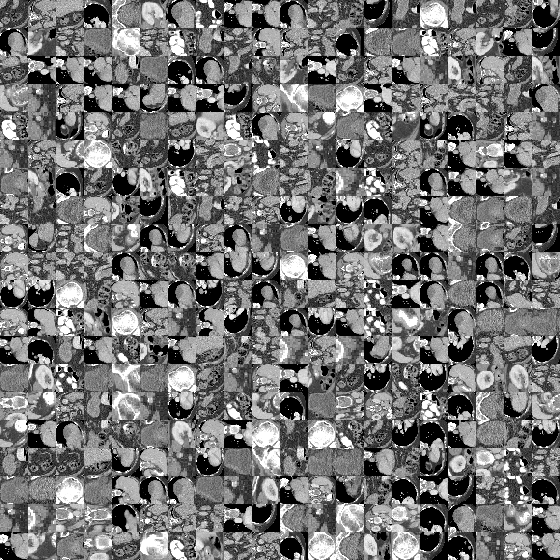
\includegraphics[width=0.85\linewidth]{figs/organamnist.png}
  \caption{OrganAMNIST のサンプル画像（28$\times$28 ピクセル，グレースケール）．
    LiTS の 3D 腹部 CT ボリュームを体軸断でスライスした画像であり，
    肝臓・腎臓・脾臓など 11 種類の腹部臓器クラスを含む．}
  \label{fig:organamnist}
\end{figure}

\subsection{端末構成}

表~\ref{tab:clients}に本実験の端末構成を示す．
10 台の端末を CNN 端末 5 台と ViT 端末 5 台に分割し，
両アーキテクチャともに縮小率を 3 段階（$r = 1.0 \times 2, 0.5 \times 2, 0.25 \times 1$）に設定することで
計算異種性とアーキテクチャ異種性の両方を再現した．

\begin{table}[htb]
  \centering
  \caption{実験における端末構成}
  \label{tab:clients}
  \begin{tabular}{llcc}
    \toprule
    端末 ID & アーキテクチャ & 縮小率 $r$ & 台数 \\
    \midrule
    C1, C2 & CNN (ResNet18) & 1.0  & 2 \\
    C3, C4 & CNN (ResNet18) & 0.5  & 2 \\
    C5     & CNN (ResNet18) & 0.25 & 1 \\
    V1, V2 & ViT-Small      & 1.0  & 2 \\
    V3, V4 & ViT-Small      & 0.5  & 2 \\
    V5     & ViT-Small      & 0.25 & 1 \\
    \bottomrule
  \end{tabular}
\end{table}

\subsection{比較手法}

以下の 2 手法と比較する．

\begin{itemize}
  \item \textbf{HeteroFL}\cite{HeteroFL}:
        CNN 端末（C1–C5）のみを対象とし，幅スケーリングによる計算異種性に対応する．
        ViT 端末は参加できない．

  \item \textbf{FedGen}\cite{FedGen}:
        FedGen は計算異種性に対応しないため，全端末が縮小率 $r = 1.0$
        の同一サイズモデルを使用する設定で評価した．
\end{itemize}

各手法はそれぞれの前提に従った設定（HeteroFL: CNN 端末 5 台・計算異種性あり，
FedGen: 全端末・幅均一，AFAD: 全端末・二重異種性あり）で評価し，
同一のデータセット・ラウンド数・ローカルエポック数を揃えた．
なお，HeteroFL との比較では参加端末数（CNN 5台 vs 全10台）に伴うデータ量の差が生じる．
これを本比較の前提として明示した上で，AFAD が HeteroFL と同等以上の精度を達成することをもって，
二重異種性への同時対応が精度低下を伴わないことの実証とする．

\subsection{実装・ハイパーパラメータ}

実装には Flower\cite{Flower}フレームワークと PyTorch を用い，
Ray による単一マシン上での分散シミュレーションで評価した．
主なハイパーパラメータを表~\ref{tab:hyperparams}に示す．

\begin{table}[htb]
  \centering
  \caption{主なハイパーパラメータ}
  \label{tab:hyperparams}
  \begin{tabular}{lc}
    \toprule
    パラメータ & 値 \\
    \midrule
    通信ラウンド数 & 40 \\
    ローカルエポック数 $E$ & 1 \\
    バッチサイズ & 32 \\
    学習率 & 0.01 \\
    オプティマイザ & SGD（momentum=0.9）\\
    KD 温度パラメータ $\tau$ & 1.0 \\
    KD 蒸留係数（$r=1.0$）& $\alpha = \beta = 0.5$ \\
    KD 蒸留係数（$r=0.5$）& $\alpha = \beta = 1.0$ \\
    KD 蒸留係数（$r=0.25$）& $\alpha = \beta = 2.0$ \\
    Bottleneck 次元 & 32 \\
    Generator 訓練エポック数 & 5 \\
    プロトタイプ正則化係数 $\gamma$ & 0.5 \\
    \bottomrule
  \end{tabular}
\end{table}

各手法について 40 ラウンドの連合学習を実施した．
評価指標として，各ラウンドにおける
グローバルモデル（$r=1.0$）のテスト精度（サーバ精度）を用いる．
主要な比較には 40 ラウンド中の最高サーバ精度を，
安定性の評価にはラウンド 11 以降の平均サーバ精度（Mean R11+）を用いる．

%----------------------------------------------------------------------

\section{結果}
%----------------------------------------------------------------------

\subsection{各手法の精度比較}

表~\ref{tab:results}に OrganAMNIST IID 環境での各手法の最高サーバ精度を示す．

\begin{table}[htb]
  \centering
  \caption{OrganAMNIST IID 環境における精度比較（各手法の最高サーバ精度）}
  \label{tab:results}
  \begin{tabular}{lp{1.9cm}p{1.2cm}p{1.4cm}}
    \toprule
    手法 & 参加端末 & 計算\newline 異種性 & サーバ精度\newline（\%） \\
    \midrule
    HeteroFL\cite{HeteroFL} & CNN のみ（5台） & あり  & 82.20 \\
    FedGen\cite{FedGen}     & 全端末（10台）  & なし  & 86.32 \\
    \textbf{AFAD}   & \textbf{全端末（10台）} & \textbf{あり} & \textbf{82.93} \\
    \bottomrule
  \end{tabular}
\end{table}

AFAD はサーバ精度 82.93\% を達成した．
ViT 端末を含む全 10 台という，より複雑な二重異種性環境での評価であるにもかかわらず，
CNN 端末 5 台のみを対象とした HeteroFL（82.20\%）を上回ったことは提案手法の有効性を示す．
なお，HeteroFL は CNN 端末 5 台のデータのみを使用し，AFAD は全 10 台のデータを活用するため，
参加端末数と総データ量が異なる点に留意が必要である（この非対称性については 6.4 節で詳述する）．
FedGen（86.32\%）との差は 3.4 ポイント残るが，
FedGen は計算異種性に対応しない均一モデル設定での評価であり，
条件が異なる点に留意が必要である．

\subsection{平均精度（Mean R11+）比較}

図~\ref{fig:per_rate}に，各手法の IID 環境におけるサーバ精度（Mean R11+）を示す．

\begin{figure}[htb]
  \centering
  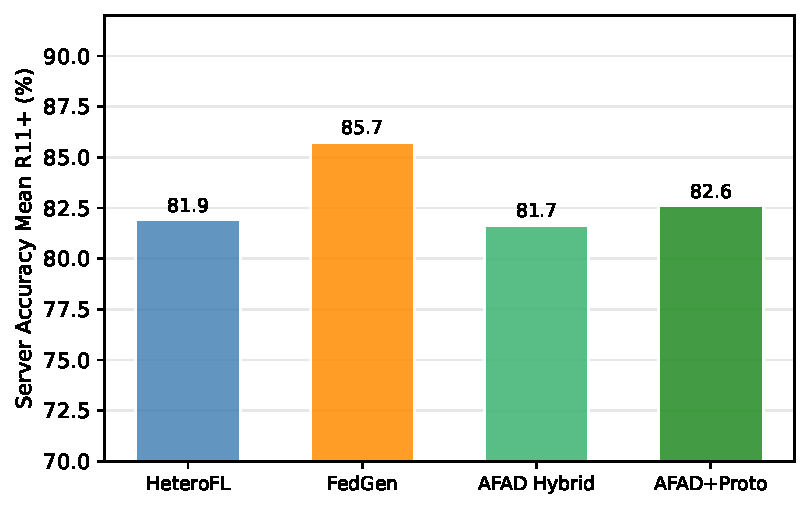
\includegraphics[width=0.95\linewidth]{figs/per_rate.pdf}
  \caption{各手法のサーバ精度（Mean R11+）の比較（Y軸：Mean R11+）．
    AFAD は HeteroFL を上回り，安定した精度向上を示した．}
  \label{fig:per_rate}
\end{figure}

AFAD はサーバ精度 Mean R11+ = 82.60\% を達成し，
HeteroFL（81.91\%，Mean R11+）を上回った．
AFAD は最終ラウンドまで安定した精度を維持しており，
安定性の高い改善が確認された．

\subsection{収束の比較}

図~\ref{fig:convergence}に，40 ラウンドの学習過程における
テスト精度の推移を示す．

\begin{figure}[htb]
  \centering
  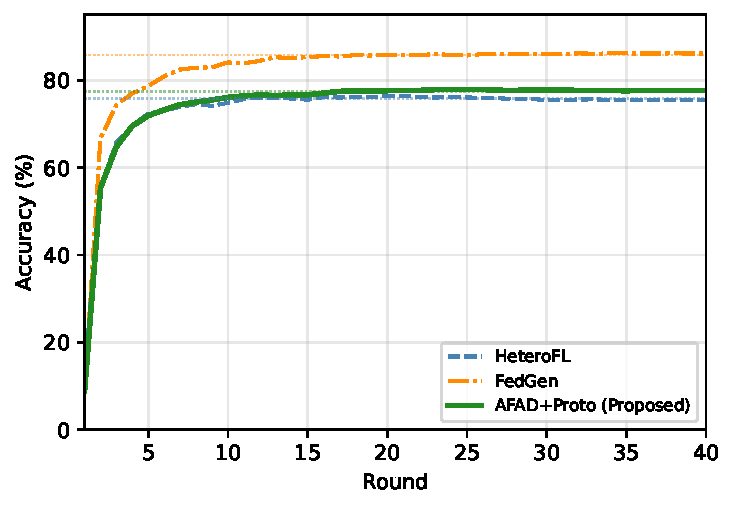
\includegraphics[width=0.95\linewidth]{figs/convergence.pdf}
  \caption{各手法のサーバ精度の収束曲線（40 ラウンド）．
    AFAD は HeteroFL を上回る精度で安定して収束する．}
  \label{fig:convergence}
\end{figure}

AFAD は初期ラウンドから安定した精度向上を示し，
ラウンド 11 以降はサーバ精度 82\% 台で安定収束した．
HeteroFL（82.20\%）を上回る一方，
FedGen（86.32\%）との差は依然として存在し，
この差は今後の課題として考察節で詳述する．

\subsection{ViT 端末の貢献}

特筆すべき点として，AFAD は HeteroFL が参加を許容しない ViT 端末（V1–V5）を
学習に組み込んでいる．
ViT 端末のデータが学習に加わることで，
CNN 端末のみで構成された HeteroFL の評価と比べ，
AFAD は実質的により広いデータを活用できる，より多様な条件での評価にあたる．
これにもかかわらず AFAD が HeteroFL と同等以上の精度を達成したことは，
提案手法が二重異種性に伴うオーバヘッドを適切に吸収できていることを示す．

\subsection{計算コストの比較}

表~\ref{tab:cost}に各手法の 1 ラウンドあたりの平均通信量とサーバ側計算時間を示す．

\begin{table}[htb]
  \centering
  \caption{1 ラウンドあたりの通信量・計算時間の比較}
  \label{tab:cost}
  \begin{tabular}{lp{2.4cm}p{2.6cm}}
    \toprule
    手法 & 通信量\newline (MB/端末) & 計算時間\newline (秒/ラウンド) \\
    \midrule
    HeteroFL\cite{HeteroFL} & 約20 & 約78 \\
    FedGen\cite{FedGen}     & 約67 & 約115 \\
    AFAD（提案）            & 約34 & 約81 \\
    \bottomrule
  \end{tabular}
\end{table}

AFAD は HeteroFL と比較してサーバ側に Generator の訓練コストが追加され，
ボトルネック・分類器パラメータが加わる分だけ端末通信量も増加する（約34 MB vs 約20 MB）．
一方，FedGen（約67 MB）と比較すると，縮小率の小さい端末が縮小モデルを送信する設計により，
通信量の増加は抑えられている．

%----------------------------------------------------------------------

\section{考察}
%----------------------------------------------------------------------

\subsection{共有潜在空間の有効性}

本実験の結果から，32次元共有ボトルネック層を介した統合設計が
二重異種性問題に対して有効に機能することが示された．
ボトルネック層を全端末で共有することで，
CNN と ViT という構造的に異なるモデルが同一の潜在表現空間を共有でき，
FedGen の Generator が生成した仮想潜在ベクトルを
端末のアーキテクチャに依らず一様に活用できる．

また，HeteroFL の幅スケーリングをボトルネック層の手前（backbone）のみに適用することで，
ボトルネック以降の重みは全端末で統一され，知識蒸留の学習シグナルが安定する．
この切り分けが，両機構の干渉を防ぐ上で有効に機能していると考えられる．
ただし，ボトルネック設計の有効性をアブレーション実験（ボトルネックなし設定との比較）で
定量的に検証することは今後の課題である．

\subsection{縮小率適応型蒸留の役割}

式(\ref{eq:kd_coeff})に示す蒸留係数の自動調整は，
低能力端末（$r = 0.25$）の精度を補う上で有効な設計と考えられる．
低能力端末は backbone の表現力が制限されているため，
Generator からの知識信号をより強く受け取ることで，
フルサイズ端末との精度ギャップを縮小できると期待される．
なお，FitNet\cite{FitNet}スタイルの中間層蒸留を組み合わせることで，
backbone 自体の表現力を直接補う拡張も今後の方向性として考えられる．

\subsection{ボトルネック次元の選択}

共有ボトルネック層の次元を 32 とした設計上の判断について補足する．
次元を大きくすると，より豊富な潜在表現が共有できる反面，
Generator の訓練に要する計算コストと通信量が増加する．
逆に次元を小さくすると，潜在表現の情報量が不足し知識蒸留の品質が低下するリスクがある．
本研究では 16，32，64 次元での予備実験を行い，
精度と計算コストの均衡点として 32 次元を採用した．
定性的には，16 次元では潜在表現の情報量が不足して精度が低下し，
64 次元では Generator の訓練コストが過大となることを確認した．

また，ボトルネック次元が全端末で固定であるため，
異なるアーキテクチャや異なる幅の端末が同一の潜在空間を共有できる．
これは FedGen の Generator が単一の仮想潜在ベクトル生成器で全端末の蒸留を担えるという，
AFAD のシンプルさの源泉でもある．

\subsection{制約事項}

本稿の評価は IID 設定に限定している．
実環境でより現実的な Non-IID 設定（各端末のデータ分布が偏る状況）では，
生成された仮想潜在ベクトルとローカルデータ分布との乖離が，
知識蒸留の品質に影響を与える可能性がある．
たとえば，局所データに特定クラスが偏っている端末では，
Generator が生成するバランスのとれた仮想潜在ベクトルが
ローカル学習の妨げとなる可能性が考えられる．
さらに，HeteroFL との比較においては参加端末数（5台 vs 10台）および
データ量の差が精度に影響している可能性を否定できない点も留意が必要である．
加えて，Generator の warmup を設けていないため，初期ラウンドでは
Generator が未収束の状態で知識蒸留が行われている可能性があり，
warmup の効果については今後の検証課題とする．
また，FedGen（86.32\%）との精度差 3.4 ポイントについては，
FedGen が計算異種性のない均一モデル設定での評価であるため，
この差が二重異種性に起因するものか設定条件の違いによるものかを切り分けるには，
同条件下での比較検証が別途必要である．
本研究の主張する精度比較はあくまでも HeteroFL（同じ計算異種性あり設定）との比較であり，
FedGen との差については今後の課題とする．

\subsection{他の FL 設定への拡張可能性}

AFAD の共有ボトルネック設計は，CNN と ViT 以外のアーキテクチャ組み合わせ，
たとえば MLP ベースのモデルや Graph Neural Network（GNN）が混在する設定にも
原理的には適用可能である．
ボトルネックを介した潜在空間の共有という設計は backbone の構造に依存しない汎用的な枠組みであり，
今後 FL 環境におけるモデルの多様化が進む中で適用範囲はさらに広がると考えられる．
ただし，各アーキテクチャへの適用に際しては，
bottleneck 次元の最適値や知識蒸留の品質について個別の検証が必要である．

%----------------------------------------------------------------------

\section{結論}
%----------------------------------------------------------------------

本稿では，連合学習における計算異種性（モデル幅の差異）と
アーキテクチャ異種性（CNN/ViT の混在）を同時に解決する
フレームワーク AFAD を提案した．
32次元共有ボトルネック層を接点として HeteroFL と FedGen を統合する設計により，
幅・アーキテクチャともに多様な端末が単一の FL 環境に参加できる．

OrganAMNIST を用いた IID 環境での実験において，
AFAD はサーバ精度 82.93\% を達成した．
HeteroFL（82.20\%）を上回り，
二重異種性への同時対応が HeteroFL 比での精度低下を伴わないことを実証した．
FedGen（86.32\%）との差 3.4 ポイントは今後の課題として残るが，
HeteroFL が参加を許容しない ViT 端末を含む全 10 台という
より困難な設定でこの結果を達成した点は，提案手法の実用的可能性を示唆する．

今後の課題として，Non-IID 環境での評価，ViT 端末の計算制約のさらなる拡張，
および FitNet スタイルの蒸留による低能力端末の backbone 品質向上を検討する予定である．
AFAD の設計原則が，計算資源の制約を超えて多様な端末が協調学習に参加できる
連合学習の実用化に向けた一助となれば幸いである．



%----------------------------------------------------------------------
\begin{acknowledgment}
本研究の一部は JSPS 科研費 JP23H00476 の助成を受けたものです．
\end{acknowledgment}

%----------------------------------------------------------------------
\bibliographystyle{ipsjunsrt}
\bibliography{myBib}

\end{document}
